% !TEX encoding = UTF-8
% !TEX TS-program = pdflatex
% !TEX root = ../tesi.tex

%**************************************************************
\chapter{Stage come tecnica aziendale}
\label{cap:tecnica-stage}
%**************************************************************

%**************************************************************
\section{Descrizione del progetto}
\label{sec:prob}
\textit{\azienda} è il primo anno che attiva progetti di stage in collaborazione con l'Università di Padova. Questo, però, non ha portato a ritardi o disagi per la mancata esperienza, da parte dell'azienda, in questo ambito. 
\subsection{Problema da risolvere per l'azienda}
Tra le tante operazioni che Smash\textregistered\ esegue, esso calcola anche la \textbf{reputazione} che un determinato utente ha.\\
Questa reputazione si suddivide nei 2 seguendi tipi:
\begin{itemize}
\item{\textbf{Reputazione totale}:} è il numero di transazioni bancarie che un determinato utente ha ricevuto.
\item{\textbf{Reputazione relativa}:} è il numero di transazione che un determinato utente ha ricevuto da un utente a scelta.
\end{itemize}
Il fattore di rischio, che Smash\textregistered\ calcola per ogni transazione, è dato anche dalla combinazione di questi 2 tipi di reputazione.\\
Fintanto che la reputazione viene calcolata su un'entità che riceve un numero modesto di transazioni giornaliere la velocità di esecuzione avviene in un tempo accettabile. 
\\Il problema emerge quando questo calcolo viene eseguito su un entità con un enorme numero di transazioni, come può essere un azienda di dominio pubblico che riceve giornalmente transazioni. Questo avviene perchè Smash\textregistered\, per calcolare la reputazione, deve caricare totalmente nella memoria il documento contenente tutte le transazioni di quella determinata azienda.
\subsection{Possibile soluzione}
Il problema potrebbe risolversi utilizzando un determinato tipo di base di dati organizata a \textbf{grafo}.\\
Un grafo è un insieme di \textbf{nodi} che possono essere collegati tra loro attraverso delle relazioni chiamate \textbf{archi}.\\
Questi tipi di base di dati riescono a rappresentare le informazioni utilizzando solamente nodi e archi.
\newpage
\begin{figure}[h!]
	\centering
	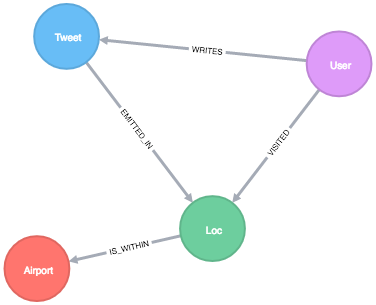
\includegraphics[scale=0.7]{immagini/grafo.png}
	\caption{\textit{Esempio grafo orientato} (\link{https://goo.gl/Z7S8J5)}}
\end{figure}
Un \textbf{nodo} può rappresentare un entità fisica come ad esempio una persona o, in questo preciso contesto, un utente di una banca. Al contrario un \textbf{arco} rappresenta una relazione che avviene tra un nodo ed un altro, come ad esempio una transazione bancaria. Qualsiasi \textbf{nodo} ed \textbf{arco} possono avere un numero a piacere di proprietà, formate da una chiave univoca ed un preciso valore. Inoltre gli \textbf{archi} possono avere un verso di relazione ed un valore che rappresenta il tipo di relazione che l'arco descrive.\\
\textbf{Se l'operazione che calcola la reputazione usasse una rappresentazione dei dati sfruttando la natura dei grafi, il calcolo della reputazione banalmente potrebbe ridursi a contare gli archi entranti di un determinato nodo.} Questo calcolo potrebbe non dipendere dal numero di transazioni che una determinata entità ha ricevuto.\\
Nella figura \hyperref[fig:figura 2.2]{2.2} \textit{Luca} avrebbe una reputazione totale pari a 3 ed una reputazione relativa, rispetto a \textit{Giovanni}, pari a 2.
\begin{figure}[h!]
	\centering
	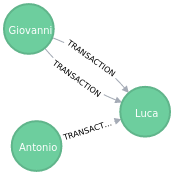
\includegraphics[scale=0.8]{immagini/grafo1.png}
	\label{fig:figura 2.2}
	\caption{\textit{Possibile implementazione della base di dati}}
\end{figure}
\label{sec:pianodl}
\subsection{Direttive del progetto di stage}
Il mio tutor aziendale, \textit{Giuseppe Pavan}, mi ha incaricato di svolgere un'analisi sulle principali tecnologie che adottano una base di dati a grafo e , successivamente, sviluppare un prototipo che cercasse di risolvere il problema precedentemente descritto.\\
L'unico vingolo imposto dal mio tutor aziendale è l'utilizzo del linguaggio Java, visto l'uso massiccio che ne fa Smash\textregistered.\\
Gli obiettivi sono stati suddivisi dal mio tutor aziendale in due categorie: obbligatori e facoltativi.\\
\\
Gli \textbf{obiettivi obbligatori} sono:
\begin{itemize}
\item{\textbf{Documentazione}:} sviluppare un documento contenente la descrizione dettagliata del lavoro di valutazione e identificazione delle soluzioni disponibili in ambito delle base di dati a grafo. Il documento descriverà i vari \textit{software} valutati, caratteristiche, vincoli e i razionali rispetto le scelte affrontate.
\item{\textbf{Ambiente Docker\glsfirstoccur}:} predisposizione di un ambiente di lavoro, con le tecnologie scelte, tramite \textit{container Docker}.
\item{\textbf{Sviluppo prototipo}:} sviluppo di una applicazione prototipale in Java che esemplifichi, partendo da un \textit{dataset} di esempio, le capacità relazionali e prestazionali delle tecnologie scelte.
\end{itemize}

Gli \textbf{obiettivi facoltativi} sono:
\begin{itemize}
\item{\textbf{Estensione del dataset}:} aggiungere maggiore complessità nel \textit{dataset} d'esempio.
\item{\textbf{Presentazione}:} preparazione di una presentazione interna da esporre al \textit{team} focalizzato sull'ambito anti frode.
\end{itemize}
\newpage
\subsection{Pianificazione}
\label{sec:pian}
La pianificazione del progetto di stage l'ha eseguita il mio tutor aziendale nel seguente modo:

\label{tab:pian}
\begin{table}[!ht]

\begin{tabularx}{\textwidth}{lXl}
\hline\hline
\textbf{Giorni} & \textbf{Attività} \\
\hline
3	& Introduzione ad ambito anti-frode focalizzato su transazioni di pagamento (descrizione degli scenari d'uso, delle tipologie di transazioni, attori coinvolti, aspetti di sicurezza e scenari di attacco)\\
\hline
2	& Definizione del problema di correlazione delle transazioni di pagamento e definizione dei requisiti\\
\hline
9	& Analisi dello stato dell'arte relativo alla tecnologia di dase di dati a grafo: identificazione delle diverse tecnologie disponibili, analisi degli elementi differenti, analisi dei requisiti e documentazione\\
\hline
5	& Progettazione del prototipo dimostrativo sfruttando soluzione proposta\\
\hline
15	& Implementazione della soluzione\\
\hline
3	& Validazione e test \\
\hline
2	 & Documentazione\\
\hline
1	& Presentazione interna dell'attività svolta\\
\hline
\end{tabularx}
\\
\caption{Tabella della pianificazione del progetto di stage}
\end{table}%



\begin{figure}[h!]
	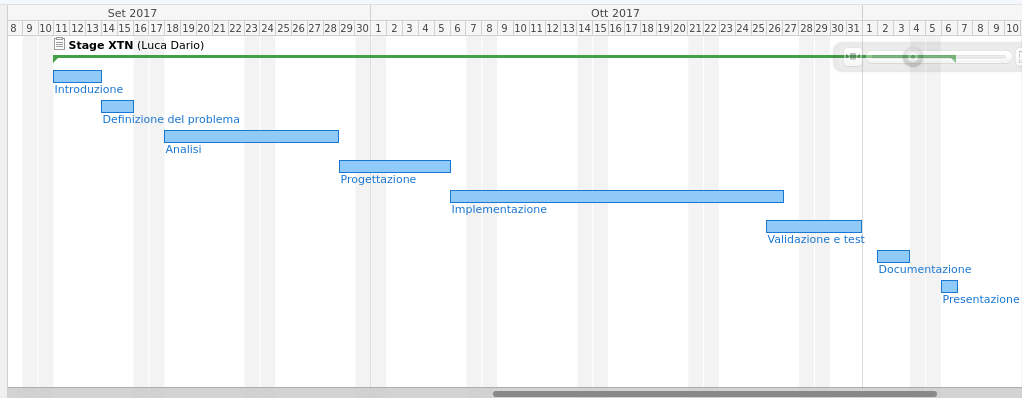
\includegraphics[scale=0.4]{immagini/gant.png}
	\caption{\textit{Diagramma di Gantt della pianificazione del progetto di stage}}
\end{figure}
La pianificazione descritta nella \hyperref[tab:pian]{tabella 2.1} soddisfa, quindi, i vincoli di durata attestandosi sui 40 giorni lavorativi corrispondenti a 320 ore.\\
\subsection{Metodologia e interazione con il tutor aziendale}
Ho deciso, in comune accordo con il tutor aziendale, che l'attività di stage dovesse essere svolta in loco presso la sede di Padova. Questo, oltre a favorire il dialogo con il tutor interno, da l'opportunità di confrontarsi assieme ad un personale con esperienza decennale nel campo dello sviluppo ed anti frode.
\newpage

\section{Aspettative aziendali}
Grazie al progetto di stage l'azienda spera di ricevere un'accurata analisi ed una possibile soluzione al problema affrontato precentemente. Questo servirà in futuro come inizio di un \textbf{analisi di fattibilità} per verificare la possibilità di adottare le tecnologie affrontate anche nei loro prodotti. Un'analisi di questo genere in un azienda rischierebbe di avere una priorità di esecuzione bassa con il rischio che questa attività non venga mai eseguita. Grazie al progetto di stage questo problema verrebbe soppiantato, insieme ad  un grosso abbattimento dei costi.

\section{Aspettative personali}
I miei obbiettivi iniziali prima della scelta del progetto di stage erano:
\begin{itemize}
\item conoscere nuove tecnologie.
\item entrare a contatto con le dinamiche del mondo del lavoro.
\item poter offrire un contributo concreto ed utile all'azienda che mi ospitava.
\item condurre un buon stage per poter sviluppare una buona tesi.
\end{itemize}
Considerando i miei obiettivi e la lista delle aziende iscritte a \textit{Stage-It}, ho deciso di scegliere questo progetto in particolare per la sua natura. Questo offre un buon compromesso tra ore spese per l'analisi ed ore per la progettazione e sviluppo. Le ore spese nell'analisi, oltre ad un \textbf{arricchimento personale}, mi permettono di scrivere una \textbf{buona tesi}. Invece le ore spese nello sviluppo mi permettono di \textbf{accrescere le mie conoscenze tecniche e di dinamiche aziendali}. \\
Successivamente alla mia scelta i miei obiettivi aumentarono, anche grazie al tema trattato dal progetto, tra cui:
\begin{itemize}
\item Mettersi in gioco per cercare di concludere tutti gli obiettivi del piano di lavoro nel miglior modo possibile. Questo mi permetterebbe di eseguire una buona presentazione del lavoro svolto in azienda.
\item Conoscere le dinamiche di rilevazione di una frode bancaria.
\item Lavorare con persone con esperienza decennale.
\item Sviluppare conoscenze in un ambito nuovo, tra cui base di dati a grafo e \textit{framework avanzati}.
\item Essere d'aiuto per risolvere un problema reale ad un azienda significativa nel loro settore.
\end{itemize}






